\documentclass[twocolumn]{article}

\title{Assignment Data Mining}
\author{Lars Moons}

\usepackage{graphicx}
\usepackage{hyperref}
\usepackage[bottom]{footmisc}

\newcommand{\attr}[1]{\texttt{#1}}

\begin{document}

\maketitle

\section{Introduction}

    The objective of this assignment is to identify potential customers for a company in order to maximise revenue. To achieve this, we must classify customers and estimate the potential profit generated from them. We will employ classification techniques using the Scikit-learn library.

\section{Exploration}

    \paragraph{Basic Statistics}
    We begin by exploring the dataset and obtaining basic statistics.
    The dataset contains 32561 rows and 15 attributes,
    including categorical and numerical attributes.
    We identified the target variable "class".

    \paragraph{Representative}
    It is essential that the historical dataset (existing customers)
    is representative of the current dataset (potential customers).
    Therefore, we validated this using the Under-Sampling technique in the Representative Notebook
    \footnote{https://github.com/lbm98/data-mining/blob/master/assignment/representative.ipynb}.
    We made barplots for all categorical attributes
    and boxplots for all numerical attributes.
    We observed that the plots all match,
    indicating that the historical dataset is representative of the current dataset.
    

\section{Preprocessing}
    In the preprocessing section, we describe the steps taken
    to prepare the dataset for further analysis.
    The Adult Notebook
    \footnote{https://github.com/lbm98/data-mining/blob/master/assignment/adult.ipynb}
    provides a guide for reproducing our results.

    \paragraph{Imbalanced Dataset}
    During exploration, we observed that the dataset is imbalanced,
    with a ratio of low-income people to high-income people of 3 to 1,
    as shown in Figure \ref{imbalance}.
    To address this issue, we used a Random Oversampling technique
    to randomly duplicate samples from the minority class
    until it had the same number of samples as the majority class.
    This technique helped to improve the performance of our models, but we need to be cautious about overfitting.

    \begin{figure}[htbp]
        \centerline{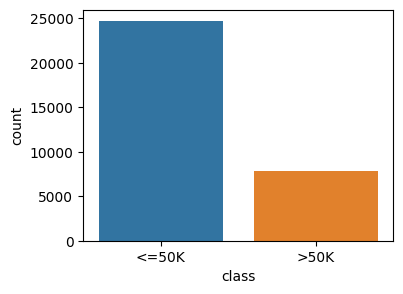
\includegraphics[width=0.7\columnwidth]{images/imbalance.png}}
        \caption{Frequency distribution of income classes}
        \label{imbalance}
    \end{figure}

    \paragraph{Redundant Attributes}
    We removed the \attr{RowID} attribute, which was completely redundant,
    and the \attr{education} attribute,
    which was perfectly correlated with \attr{eduction-num}.
    We also converted the target attribute \attr{class} into a binary format
    by assigning low-income a value of 0 and high-income a value of 1.

    \paragraph{Missing Values}
    We handled missing values in the attributes
    \attr{workclass}, \attr{occupation} and \attr{native-country}
    using different techniques.
    For \attr{workclass} and \attr{native-country}, we imputed the missing value with the most frequent value since their values were not evenly distributed but centered around one value. In contrast, for \attr{occupation}, which was more evenly distributed, we used a more advanced imputing strategy that sampled the missing values according to a distribution based on the values' frequency of occurrence.

    \paragraph{Outliers}
    We identified outliers in the \attr{capital-gain} and \attr{capital-loss} attributes, with more than 90\% of their values being 0.
    While their means are nearly 0, these attributes also include some outliers with large values.
    We normalised both attributes to reduce the impact of these outliers.

    \begin{figure}[htbp]
        \centerline{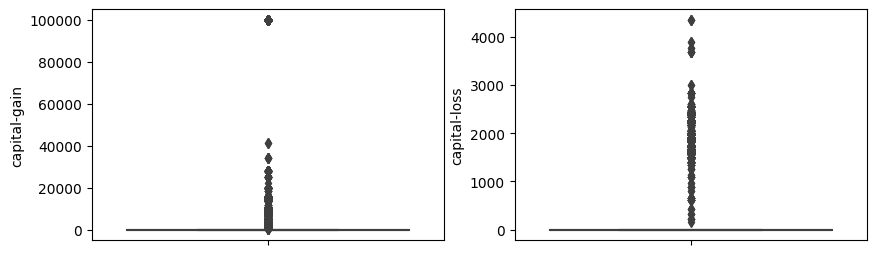
\includegraphics[width=\columnwidth]{images/outliers.png}}
        \caption{Boxplot of capital-gain and capital-loss}
        \label{outliers}
    \end{figure}

    \paragraph{Categorical Attributes}
    Finally, we converted the categorical attributes to numerical attributes using one-hot encoding since none of the attributes carried a notion of order.
    However, we were careful when dealing with attributes with a high cardinality, such as \attr{native-country}, which had 41 possible values,
    but nearly all entries presented the same value, United-States.
    Hence, we limited the number of categories to 3, resulting in a total of 51 categories.

\section{Machine Learning}

    \paragraph{Decision Tree}
    We evaluated three machine learning algorithms for our classification task, starting with Decision Trees. We began by extracting the target attribute, \attr{class}, and splitting the dataset into training and test data. We then conducted a hyperparameter search to determine the optimal maximum depth of the tree. The range of possible depths was set from 1 to 60 with some small gaps in between. We were careful to avoid the common pitfall of incorrectly holding out the data during hyperparameter optimisation. The Decision Tree model achieved an accuracy of 89.63\% with the confusion matrix shown in Figure \ref{dt-cm}. The promising results prompted us to plot the ROC curve, which is illustrated in Figure \ref{dt-roc}.

    \begin{figure}[htbp]
        \centerline{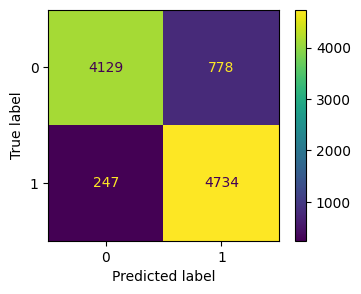
\includegraphics[width=0.6\columnwidth]{images/dt-cm.png}}
        \caption{Confusion matrix of Decision Tree model}
        \label{dt-cm}
    \end{figure}

    \begin{figure}[htbp]
        \centerline{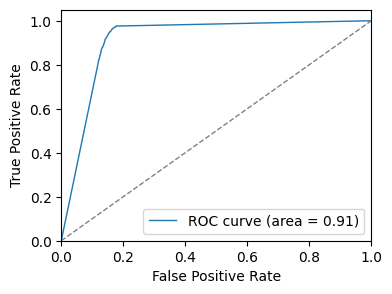
\includegraphics[width=0.7\columnwidth]{images/dt-roc.png}}
        \caption{ROC curve of Decision Tree model}
        \label{dt-roc}
    \end{figure}

    \paragraph{Model Evaluation}
    In addition to Decision Trees, we also experimented with Gaussian Naive Bayes and Logistic Regression models. However, both performed worse than the Decision Tree model. Table \ref{model_performance} summarises the main evaluation metrics, including accuracy, precision, recall, F1 score, total profit, and profit per person, for each of the three models. As shown, the Decision Tree model achieved the highest accuracy and F1 score, and also yielded the highest total profit and profit per person. Thus, we decided to choose it as the final model for our classification task.

    \begin{table*}[htbp]
        \centering
        \small
        \caption{Classification Model Performance Summary}
        \label{model_performance}
        \begin{tabular}{|c|c|c|c|c|c|c|}
        \hline
        \textbf{Model} & \textbf{Accuracy} & \textbf{Precision} & \textbf{Recall} & \textbf{F1 Score} & \textbf{Total Profit} & \textbf{Profit per person}\\ \hline
        Decision Tree        & 89.63 & 0.86 & 0.95 & 0.90 & 396753.00 & 40.12 \\ \hline
        Gaussian NB          & 76.00 & 0.70 & 0.92 & 0.79 & 352816.50 & 35.68 \\ \hline
        Logistic Regression  & 82.02 & 0.81 & 0.84 & 0.82 & 341801.50 & 34.57 \\ \hline
        \end{tabular}
    \end{table*}

\section{Profit Estimation}

    \paragraph{Profit Model}
    Our main objective is to maximise revenue, which requires targeting promotions to high-income individuals.
    This is because only high-income individuals have the potential to contribute positively to our revenue.
    With this objective in mind, we developed a profit model using the following formula:

    \small
    \[
        \mathrm{PROFIT} = \mathrm{FP} (-10 + \frac{5}{100} (-310)) + \mathrm{TP} (-10 + \frac{10}{100} 980)
    \]
    \normalsize

    Here, $\mathrm{FP}$ refers to the number of false positives, and $\mathrm{TP}$ refers to the number of true positives. The first term captures the return from the actual low-income individuals who were incorrectly identified as high-income, while the second term captures the return from the actual high-income individuals who were correctly identified. We will mostly be interested in a variation of this formula, the profit-per-entry, which is defined as follows:

    \small
    \[
        \mathrm{PROFIT\_PER\_ENTRY} = \frac{\mathrm{PROFIT}}{\mathrm{\#ENTRIES}}
    \]
    \normalsize

    \paragraph{Decision Threshold}
    Using the profit-per-entry formula, we can determine the optimal threshold for our Decision Tree model. Figure \ref{threshold-gain} shows the profit-per-entry as a function of the threshold. We found that the maximum profit-per-entry is 41 Euros and can be achieved at a threshold of 0.01.

    \begin{figure}[htbp]
        \centerline{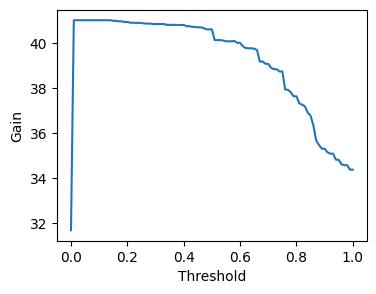
\includegraphics[width=0.7\columnwidth]{images/threshold-gain.png}}
        \caption{Profit-per-entry in function of the threshold}
        \label{threshold-gain}
    \end{figure}

\section{Predicting}
    The final step in this process involves making predictions. We begin by preparing the potential-customer dataset using methods similar to those used in previous sections, ensuring that our model can properly process the data. We then obtain prediction probabilities, which are presented in a two-column array: the first column represents the probability of a low-income individual, while the second column represents the probability of a high-income individual. We apply a decision threshold to this array, resulting in final statistics.

\section{Conclusion}
    In conclusion, out of the total of 16,281 potential customers, our model predicts that 4,737 individuals have a high income and should receive promotions to maximise revenue from the campaign. Based on an estimated profit of 41 Euro per person, we anticipate a total profit of 194,217 Euro. To find the indices of the individuals who should receive promotions, please refer to this file
    \footnote{https://github.com/lbm98/data-mining/blob/master/assignment/indices.csv}.
    
\end{document}
